\chapter{Algorithm optimization}
\label{chap:opt}

We did not want our results to be dependent on the specific classifier or regressor selected to the task. Thus, we compared the performance of some classifiers and regressors, with both their default parameters and with hyperparameters tuned. Results are shown in figures \ref{fig:clf_comparison} and \ref{fig:reg_comparison}. Because the tuning procedure took much computation, we did not repeat it with multiple training and test sets.

Half of the trials were separated for the tuning/training set, while trials from the other half were used for evaluation of the final score. We calculated scores in each tuning step with 5 folds of Monte Carlo cross validation, and afterwards trained on the full half to evaluate the model in the remaining half.
    
\begin{figure}[ht]
        \centering
        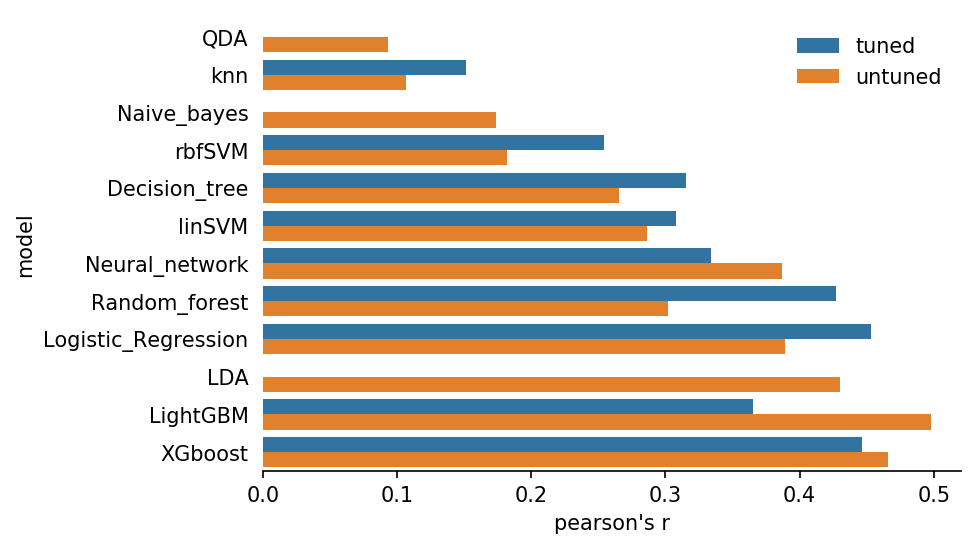
\includegraphics[width=0.9\textwidth]{figures/plots/classifier_hyperopt.png}
        \caption[Comparison of classifiers]{Comparison of classifiers. Default hyperparameters were compared with those resulting from tuning when there were hyperparameters to tune.}
        \label{fig:clf_comparison}
\end{figure}

We found big differences in performance between the multiple classifiers tested. Some classifiers have good results out-of-the-box, such as Logistic Regression and Linear Discriminant Analysis (LDA), while some are highly dependent on hyperparameter tuning, such as Random Forest. On the other hand, the capacity to decode the activity is not specific to specific algorithms, and the differences in performance are expected. The two better ranked classifiers were the Gradient Boosting Machines (GBMs), the most widely applied classifiers in online machine learning competitions \cite{chen2016xgboost, ke2017lightgbm}. The same occurred for the regressors, with the boosting algorithms ranking best. 

%  The results for the gradient boosting classifiers LightGBM and XGBoost are specially interesting, as they have better results on the default configurations than after tuning, which is probably due to the fact that we were tuning 10 different hyperparameters.
 
\begin{figure}[ht]
        \centering
        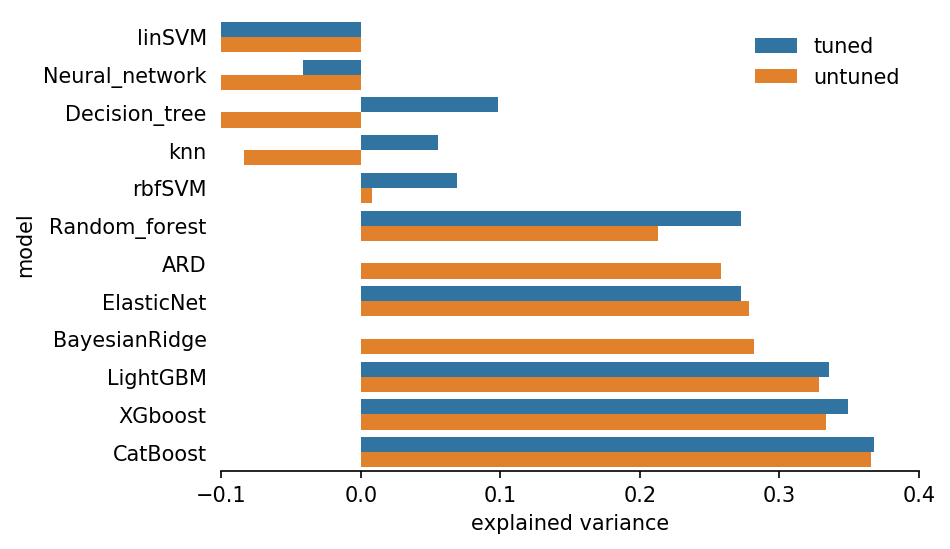
\includegraphics[width=0.9\textwidth]{figures/plots/regressor_hyperopt.png}
        \caption[Comparison of classifiers]{Comparison of regressors. Default hyperparameters were compared with those resulting from tuning when there were hyperparameters to tune.}
        \label{fig:reg_comparison}
\end{figure}

Tuning machine learning models is not as simple as it may seem, what it clear from studies that tune the model in the same data in which they measure its performance, a process that may bias up the performance of the tuned model. To understand why this is the case, we must understand the hyperparameter tuning as part of the model fitting procedure. Since we choose the hyperparameters that best perform in our hyperparameter-tuning subset (tuning set) of the data, we are biasing our results in this specific subset of data. Specially when tuning complex models with a lot of hyperparamers, such as we did with the GBMs, we risk overfitting the tuning set in the hyperparameter choice, ending up with tuned performances that are smaller than untuned performances, as in the case of GBMs for classification. In that case, we can observe that the performance was higher before than after tuning.

Interestingly, in both cases we found extremely simple algorithms ranking close to the boosting ones, specifically Linear Discriminant Analysis and Bayesian Ridge. This has been shown by a single comparison in chapter \ref{chap:opt}, but actually goes even further since our results qualitatively agree when using other classifiers (not shown here). 

From the point of view of facilitating the use of machine learning in neuroscience, this finding reduces the barrier, at least for problems that are similar to ours. Instead of spending time and resources tuning complex models, simple models even without tuning may suffice to decode the patterns of interest. 

This advice has to be taken with caution, because it does not apply to every simple model. Some of them are highly dependent on the hyperparameters, for example the Support Vector Machine and Random Forest. The Bayesian Ridge and Linear Discriminant Analysis are more robust to hyperparameter choice, and since they are explicitly Bayesian algorithms we did not even tuned hyperparameters for them. 

Further limitations of our findings are the lack of a distribution of scores. Since it was computationally expensive to tune the models, especially the boosting ones, we did the process a single time, and in the discussion we are supposing that this one result is representative. To surpass this limitation, we would need to run the hyperparameter search multiple times (e.g. 5) within a cross-validation loop.

% For most classifiers, there is significant decoding for as little as 10 trials in the training set. As expected, the classifier's performance increases with the number of trials used for training it. It is even possible that a bigger training set would give us even higher scores, pointing to the importance of having big experimental sessions with many trials. Hence, if we want to compare the information contained in the neural activity in different moments in a session, we have to ensure their classification models are trained with the same number of trials.
